\documentclass[a4paper, 10pt]{article}
\usepackage{amsmath}
\usepackage{fancyhdr}
\usepackage{float}
\usepackage[a4paper, left=1in, right=1in, top=1in, bottom=1in]{geometry} % Adjust margins
\usepackage{graphicx}
\usepackage{listings}
\usepackage{matlab-prettifier}

\pagestyle{fancy}

\title{ECE 340 Lab 2}
\author{Omar Mahmoud\\1753607\\Section D21}
\date{10/10/2024}

\lhead{Omar Mahmoud}
\rhead{ECE 340 Lab 2}
\headheight 15pt

\begin{document}

%% Cover Page
\thispagestyle{empty}
\vfill
\maketitle
\vfill

\newpage

% Q1: Intro to Convolution
\section{Intro to Convolution}
Given the two discrete functions:
\begin{equation}
  x[k] =
  \begin{cases} 
  k, & 0 \leq k \leq 4\\
  0, & \text{otherwise}
  \end{cases}
\end{equation}
\begin{equation}
  h[k] =
  \begin{cases} 
  2-k, & 0 \leq k \leq 3\\
  0, & \text{otherwise}
  \end{cases}
\end{equation}
They were be plotted on the same page in MATLAB using the following code:
\begin{lstlisting}[style=Matlab-editor, basicstyle=\small\ttfamily]
  figure(1);

  % plot x[k]
  subplot(2, 1, 1);
  k = -5:10;
  x = zeros(size(k));
  x(0 <= k & k <= 4) = k(0<= k & k <= 4);
  stem(k, x, 'r', 'DisplayName' ,'x[k]');
  title('Plot of x[k]')
  xlabel('k')
  ylabel('x[k]')
  
  % plot h[k]
  subplot(2, 1, 2);
  h = zeros(size(k));
  h(0 <= k & k <= 3) = 2 - k(0 <= k & k <= 3);
  stem(k, h, 'b', 'DisplayName', 'h[k]');
  title('Plot of h[k]')
  xlabel('k')
  ylabel('h[k]')
\end{lstlisting}
\begin{figure}[H]
  \centering
  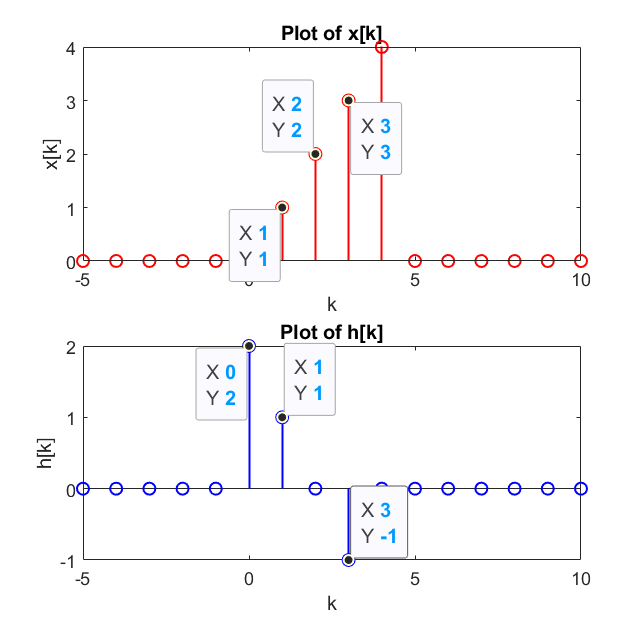
\includegraphics[width=10cm]{images/q1_given.png}
  \caption{Plot of $x[k]$ and $h[k]$ defined above.}
\end{figure}
To convolve these to functions with MATLAB's \textit{conv} function the following script was used:
\begin{lstlisting}[style=Matlab-editor, basicstyle=\small\ttfamily]
  figure(2);
  
  % convolve using 'conv' and plot the result
  subplot(2, 1, 1);
  y = conv(x, h);
  k_conv = (min(k) + min(k)) : (max(k) + max(k)); % convolution range
  stem(k_conv, y, 'LineWidth', 1, 'Color', '#036b30');
  title('Plot of x[k] * h[k], Calculated Using conv.');
  xlabel('k');
  ylabel('x[k] * h[k]'); 
\end{lstlisting}
To compare to the results of the \textit{conv} function, the convolution was computed manually with the following script:
\begin{lstlisting}[style=Matlab-editor, basicstyle=\small\ttfamily]
  % manually compute the convolution and plot the result
  subplot(2, 1, 2);
  len_x = length(x);
  len_h = length(h);
  len_y = len_x + len_h - 1;  % length of the result
  y_manual = zeros(1, len_y);
  for k = 1:len_y
    for n = 1:len_x
      if (k-n+1 > 0) && (k-n+1 <= len_h)
        y_manual(k) = y_manual(k) + x(n) * h(k-n+1);
      end
    end
  end
  stem(k_conv, y_manual, 'LineWidth', 1, 'Color', '#010a87');
  title('Plot of x[k] * h[k], Calculated Manually.');
  xlabel('k');
  xlabel('x[k] * h[k]');  
\end{lstlisting}
The results of the two convolutions were as follows.
\begin{figure}[H]
  \centering
  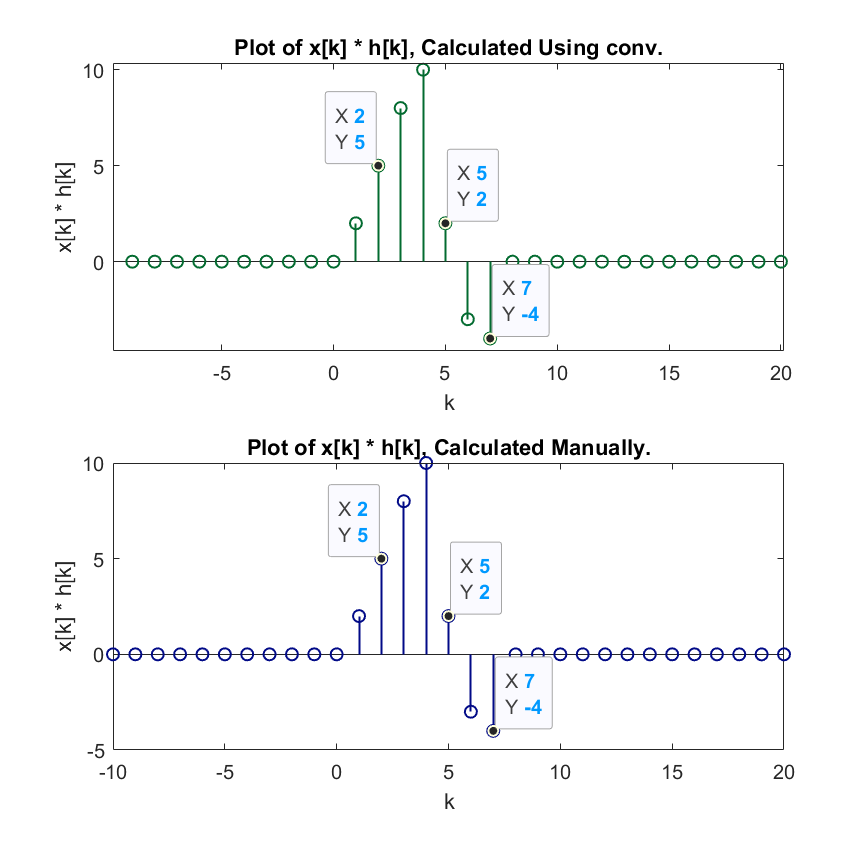
\includegraphics[width=10cm]{images/q1_result.png}
  \caption{Plot of $x[k] * h[k]$.}
\end{figure}
\noindent By checking the values of several points on both plots, it was clear that the results of the manual convolution
and the \textit{conv} match.

% Q2: Convolution of Audio
\section{Convolution of Audio}
Given a system with the following impulse response:
\begin{equation}
  h[k]  =
  \begin{cases}
    0.3\mathrm{sinc}(0.3(k-25)) \left(0.54-0.46\cos[\frac{2\pi k}{50}]\right) & 0\leq k\leq 50\\
    0 & \text{otherwise}
  \end{cases}
\end{equation}
The impulse response can be plotted using the following MATLAB script:
\begin{lstlisting}[style=Matlab-editor, basicstyle=\small\ttfamily]
  figure(1);

  % plot the impulse response h[k]
  k = -10:60;
  h = zeros(size(k));
  for i = 1:length(k)
    if 0 <= k(i) && k(i) <= 50
      h(i) = 0.3 * sinc(0.3 * (k(i) - 25)) * (0.54 - 0.46 * cos((2 * pi * k(i))/50));
    end
  end
  stem(k, h, 'LineWidth', 1, 'Color', 'r');
  title('Plot of the Impulse Response h[k].');
  xlabel('k');
  ylabel('h[k]');  
\end{lstlisting}
\begin{figure}[H]
  \centering
  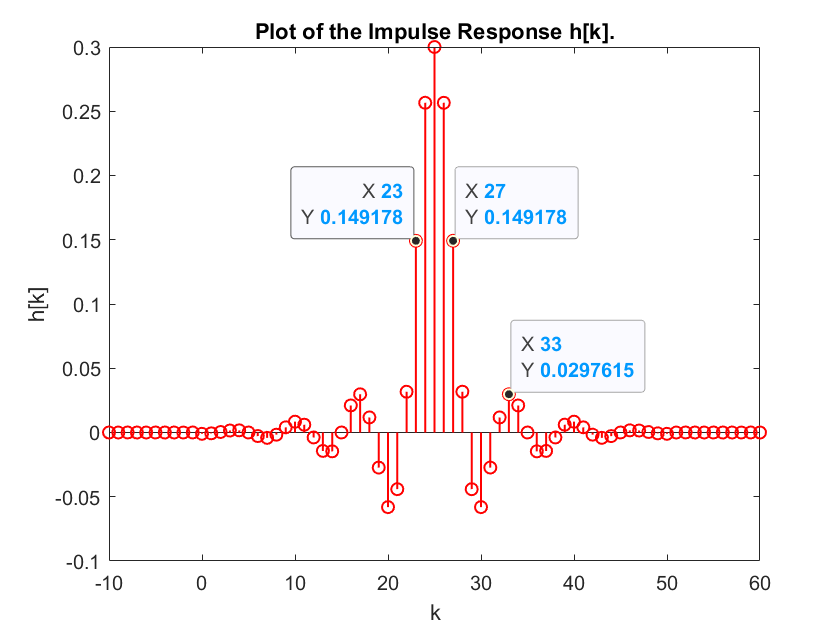
\includegraphics[width=10cm]{images/q2_impulse.png}
  \caption{Plot of the impulse response $h[k]$.}
\end{figure}
Given the audio file \textit{baila.wav}, the convolution of its signal and the impulse response $h[k]$ can 
be calculated and written to a new file \textit{baila\_filtered.wav} using the following MATLAB script:
\begin{lstlisting}[style=Matlab-editor, basicstyle=\small\ttfamily]
  % read baila.wav audio file
  [x3, Fs] = audioread('baila.wav');
  t = (0:length(x3) - 1) / Fs;
  x3f = conv(x3, h, 'same');
  audiowrite('baila_filtered.wav', x3f, Fs);
\end{lstlisting}
The result of the following convolution was a grainier and muffled version of the original \textit{baila.wav} file.

% Q3: Effects of Aliasing on 1D Sinusoidal Signals
\section{Effects of Aliasing on 1D Sinusoidal Signals}
Given the two continuous-time sinusoidal signals $x_1(t) = \cos(20\pi t)$ and $x_2(t) = \cos(180\pi t)$, along with
a sampling frequency of $f_{s_1} = 100 \, \text{Hz}$, the resulting discrete-time signals $y_1[n]$ and $y_2[n]$ for 
$0 \leq n \leq 30$ can be computed and plotted using the following MATLAB script:
\begin{lstlisting}[style=Matlab-editor, basicstyle=\small\ttfamily]
  % get y1 and y2
  fs1 = 100; % sampling frequency of 100hz
  n1 = 0:30; % index from 0 to 30
  t1 = n1 / fs1; % time-vector for continuous-time signals
  
  y1 = cos(20 * pi * t1);
  y2 = cos(180 * pi * t1);
  
  figure(1);
  
  % subplot for y1[n]
  subplot(2, 1, 1);
  stem(n1, y1, 'LineWidth', 1, 'Color', 'r');
  title('Stem Plot of y_1[n] = cos(20\pi t)');
  xlabel('n');
  ylabel('y_1[n]');
  
  % subplot for y2[n]
  subplot(2, 1, 2);
  stem(n1, y2, 'LineWidth', 1, 'Color', 'b');
  title('Stem Plot of y_2[n] = cos(180\pi t)');
  xlabel('n');
  ylabel('y_2[n]');  
\end{lstlisting}
\begin{figure}[H]
  \centering
  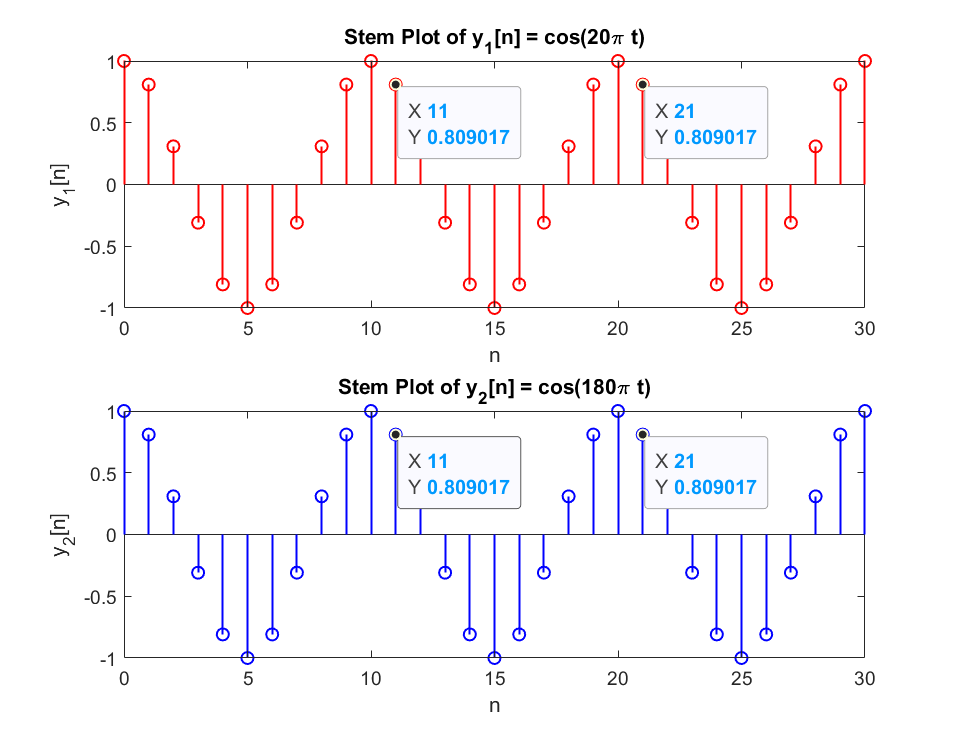
\includegraphics[width=12cm]{images/q3_a.png}
  \caption{Plots of discrete-time signals $y_1[k]$ and $y_2[k]$.}
\end{figure}
Looking at the plots side-by-side, and when several points are compared, it was clear that $y_1[n]$ and $y_2[n]$ with
a sampling frequency $f_{s_1} = 100Hz$ have an identical output. This was because $y_2[n]$ can be seen as being equal to
$y_1[n-2\pi * n]$:
\begin{center}
  $y_2[n] = \cos(\frac{20\pi n}{100} - \frac{200\pi n}{100}) = \cos(\frac{180\pi n}{100})$
\end{center}

\hfill

\noindent If the sampling frequency of $x_1(t)$ and $x_2(t)$ was set to $f_{s_2}=1000Hz$, the resulting discrete-time signals
$z_1[n]$ and $z_2[n]$ for $0\leq n\leq 300$ can be calculated and plotted using the following MATLAB script:
\begin{lstlisting}[style=Matlab-editor, basicstyle=\small\ttfamily]
  % plot z1 and z2
  figure(2);
  
  fs2 = 1000; % sampling frequency of 100hz
  n2 = 0:300; % Time index for z1 and z2
  t2 = n2 / fs2;
  
  z1 = cos(20 * pi * t2);
  z2 = cos(180 * pi * t2);
  
  % subplot for z1[n]
  subplot(2, 1, 1);
  stem(n2, z1, 'LineWidth', 1, 'Color', 'r');
  title('Stem Plot of z_1[n] = cos(20\pi t)');
  xlabel('n');
  ylabel('z_1[n]');
  
  % subplot for z2[n]
  subplot(2, 1, 2);
  stem(n2, z2, 'LineWidth', 1, 'Color', 'b');
  title('Stem Plot of z_2[n] = cos(180\pi t)');
  xlabel('n');
  ylabel('z_2[n]');  
\end{lstlisting}
\begin{figure}[H]
  \centering
  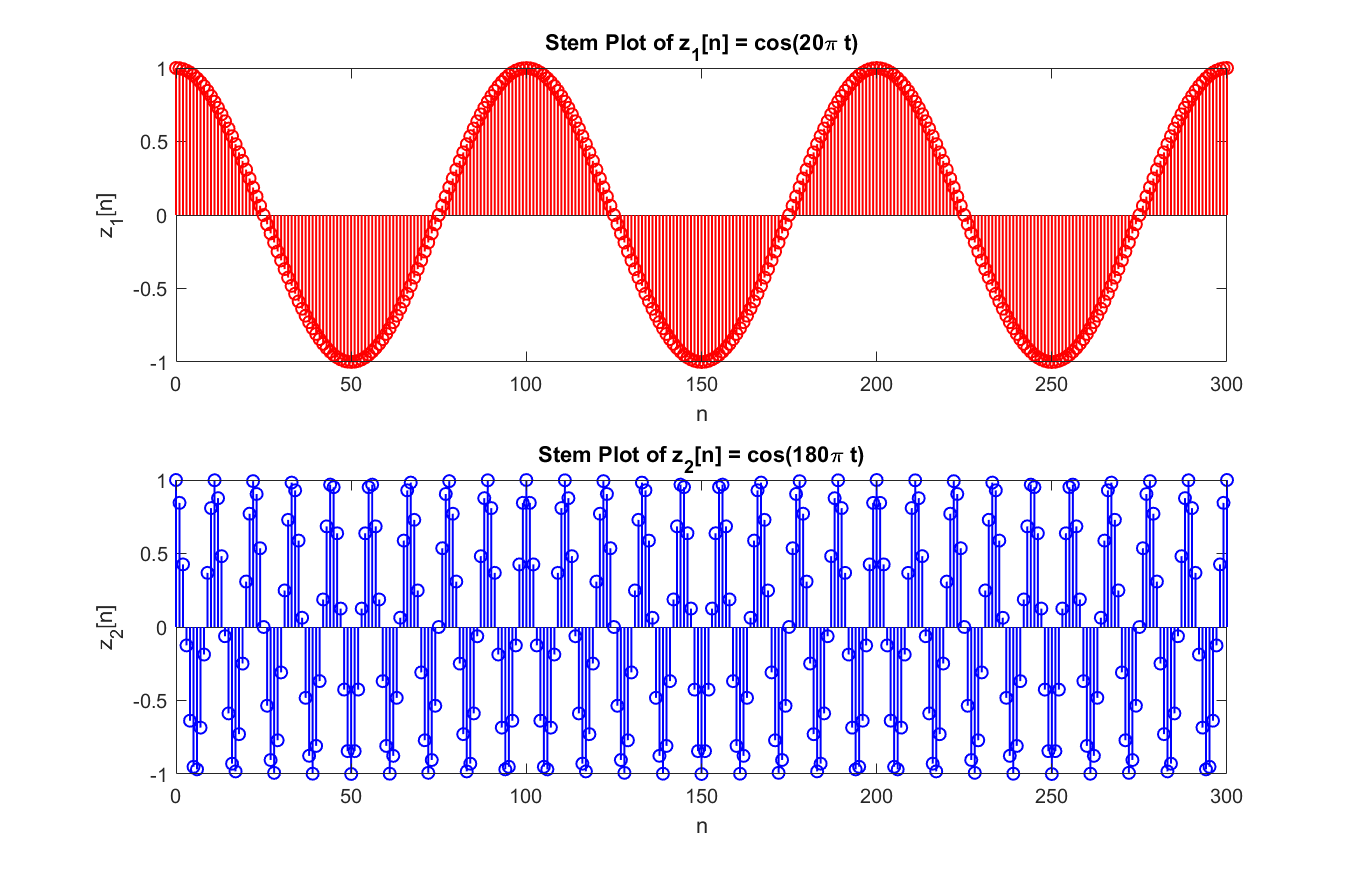
\includegraphics[width=14cm]{images/q3_z.png}
  \caption{Plot of $y_1[n]$ and $z_1[n]$, and $y_1[n]$ and $z_1[n]$}
\end{figure}
Now to compare $y_1[n]$ and $y_2[n]$ with $z_1[n]$ with $z_2[n]$ by plotting them togther using the following MATLAB code:
\begin{lstlisting}[style=Matlab-editor, basicstyle=\small\ttfamily]
  % plotting z1 and y1 and z2 and y2
  figure(3)
  % Create the first subplot
  subplot(2,1,1);
  plot(n2/fs2, z1, 'r-', n1/fs1, y1, 'b+', 'LineWidth', 1);
  xlabel('n'); ylabel('y_1[n] and z_1[n]');
  legend('z_1[n]', 'y_1[n]');
  title('Plot of y_1[n] and z_1[n]');
  
  % Create the second subplot
  subplot(2,1,2);
  plot(n2/fs2, z2, 'r-', n1/fs1, y2, 'b+', 'LineWidth', 1);
  xlabel('n'); ylabel('y_2[n] and z_2[n]');
  legend('z_2[n]', 'y_2[n]');
  title('Plot of y_2[n] and z_2[n]');
\end{lstlisting}
\begin{figure}[H]
  \centering
  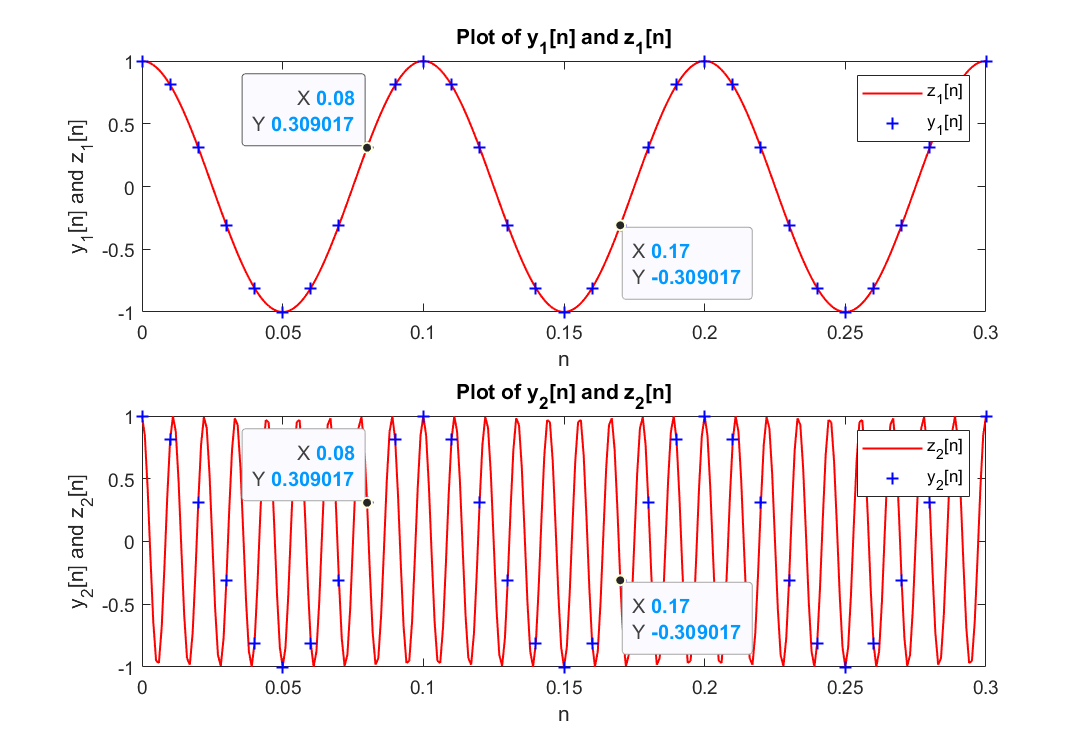
\includegraphics[width=12cm]{images/q3_b.png}
  \caption{Plot of $y_1[n]$ and $z_1[n]$, and $y_1[n]$ and $z_1[n]$}
\end{figure}
When observing the two plots, it was clear that when sampling at a lower frequency, such as $f_{s_1} = 100Hz$,
the sampling points can be spaced out far enough to make it difficult to accurately represent the system. This
illustrates the phenomenon of aliasing, where higher frequency components overlap/fold back into lower frequencies.
As a result one cannot distinguish between the higher and lower frequency signals.

\hfill

\noindent To find another continuous-time sinusoidal signal with different analog frequencies (in addition to $20\pi$ and $180\pi$)
whose discrete-time signal $y_3[n]$ will be the same as $y_1[n]$ after sampling with a frequency of $f_s = 100Hz$, a 
period shift can be performed:
\begin{center}
  $y_3[n] = \cos(\frac{20\pi n}{100} + 2\pi n * \frac{100}{100}) = cos(\frac{220\pi n}{100}) \rightarrow x_3(t) = \cos(220\pi t)$
\end{center}
To confirm that $y_3[n]$ was identical to $y_1[n]$ the following MATLAB script was ran:
\begin{lstlisting}[style=Matlab-editor, basicstyle=\small\ttfamily]
  figure(4)

  % plot y3
  y3 = cos(220 * pi * t1);
  subplot(2,1,1);
  stem(n1, y3, 'LineWidth', 1, 'Color', 'b');
  title('Stem Plot of y_3[n] = cos(220\pi t)');
  xlabel('n');
  ylabel('y_3[n]');
  
  % plot y1
  subplot(2,1,2);
  stem(n1, y1, 'LineWidth', 1, 'Color', 'r');
  title('Stem Plot of y_1[n] = cos(20\pi t)');
  xlabel('n');
  ylabel('y_1[n]');
\end{lstlisting}
\begin{figure}[H]
  \centering
  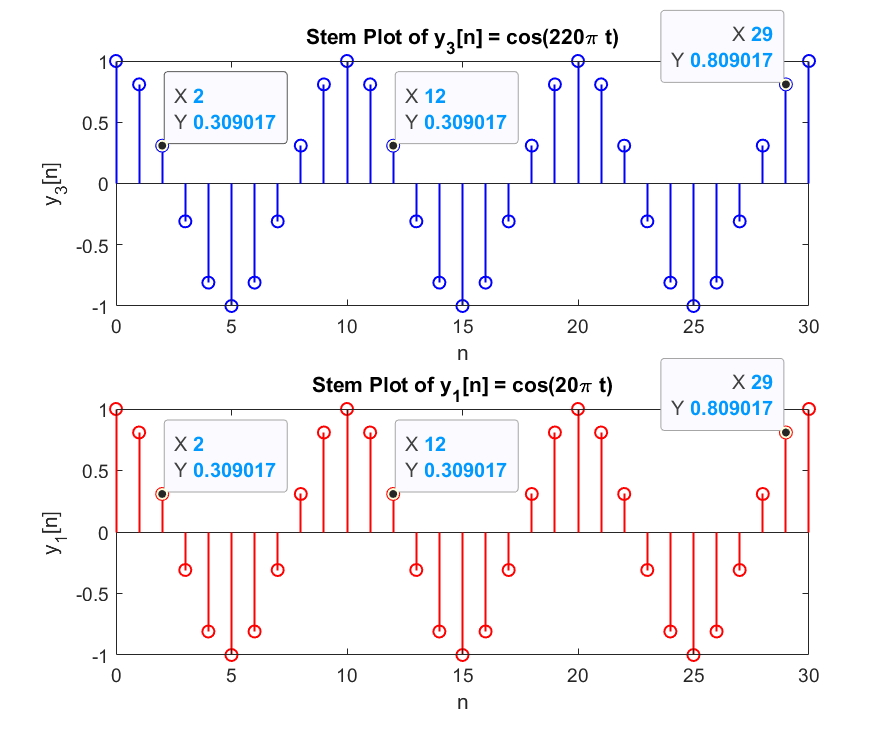
\includegraphics[width=11cm]{images/q3_c.png}
  \caption{Plot of $y_3[n]$ (top) and $y_1[n] (bottom).$}
\end{figure}
By observing both plots and comparing the values of several points, it was clear that both $y_3[n]$ and $y_1[n]$ are 
identical.

% Q4: Effects of Aliasing on 2D Signals
\section{Effects of Aliasing on 2D Signals}
Given the JPEG file \textit{barbaraLarge.jpg}, the following MATLAB script reads and displays the image alongside
its colorbar:
\begin{lstlisting}[style=Matlab-editor, basicstyle=\small\ttfamily]
  figure(1);

  % read and display the jpg file
  img = imread('barbaraLarge.jpg');
  imshow(img), colorbar;
\end{lstlisting}
\begin{figure}[H]
  \centering
  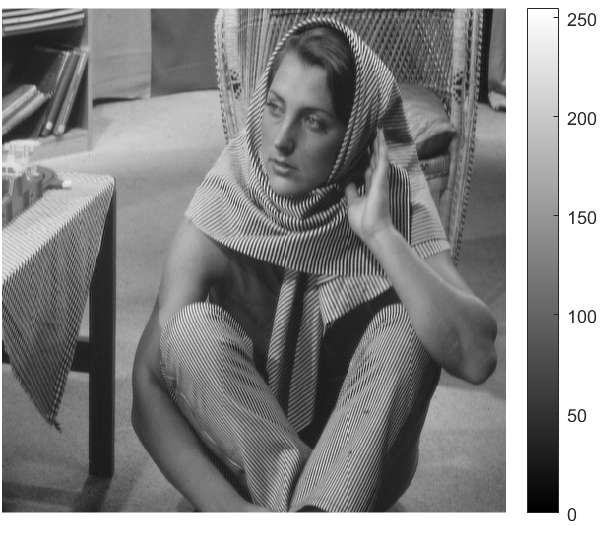
\includegraphics[width=7cm]{images/q4_ab.png}
  \caption{\textit{barbaraLarge.jpg} displayed through the above script alongside its colorbar.}
\end{figure}
To compare different resizing factors with and without anti-aliasing the following MATLAB script is ran:
\begin{lstlisting}[style=Matlab-editor, basicstyle=\small\ttfamily]
  % compare different resizing factors w/ and w/o anti-aliasing
  figure(2);
  
  subplot(2, 3, 1);
  rf = 0.9;
  img_resized = imresize(img, rf, 'nearest', 'antialiasing', 0);
  imshow(img_resized);
  title('Barbara Image w/o Anti-Alieasing and RF = 0.9');
  
  subplot(2, 3, 2);
  rf = 0.7;
  img_resized = imresize(img, rf, 'nearest', 'antialiasing', 0);
  imshow(img_resized);
  title('Barbara Image w/o Anti-Alieasing and RF = 0.7');
  
  subplot(2, 3, 3);
  rf = 0.5;
  img_resized = imresize(img, rf, 'nearest', 'antialiasing', 0);
  imshow(img_resized);
  title('Barbara Image w/o Anti-Alieasing and RF = 0.5');
  
  subplot(2, 3, 4);
  rf = 0.9;
  img_resized = imresize(img, rf, 'nearest', 'antialiasing', 1);
  imshow(img_resized);
  title('Barbara Image w/ Anti-Alieasing and RF = 0.9');
  
  subplot(2, 3, 5);
  rf = 0.7;
  img_resized = imresize(img, rf, 'nearest', 'antialiasing', 1);
  imshow(img_resized);
  title('Barbara Image w/ Anti-Alieasing and RF = 0.7');
  
  subplot(2, 3, 6);
  rf = 0.5;
  img_resized = imresize(img, rf, 'nearest', 'antialiasing', 1);
  imshow(img_resized);
  title('Barbara Image w/ Anti-Alieasing and RF = 0.5');
\end{lstlisting}
\begin{figure}[H]
  \centering
  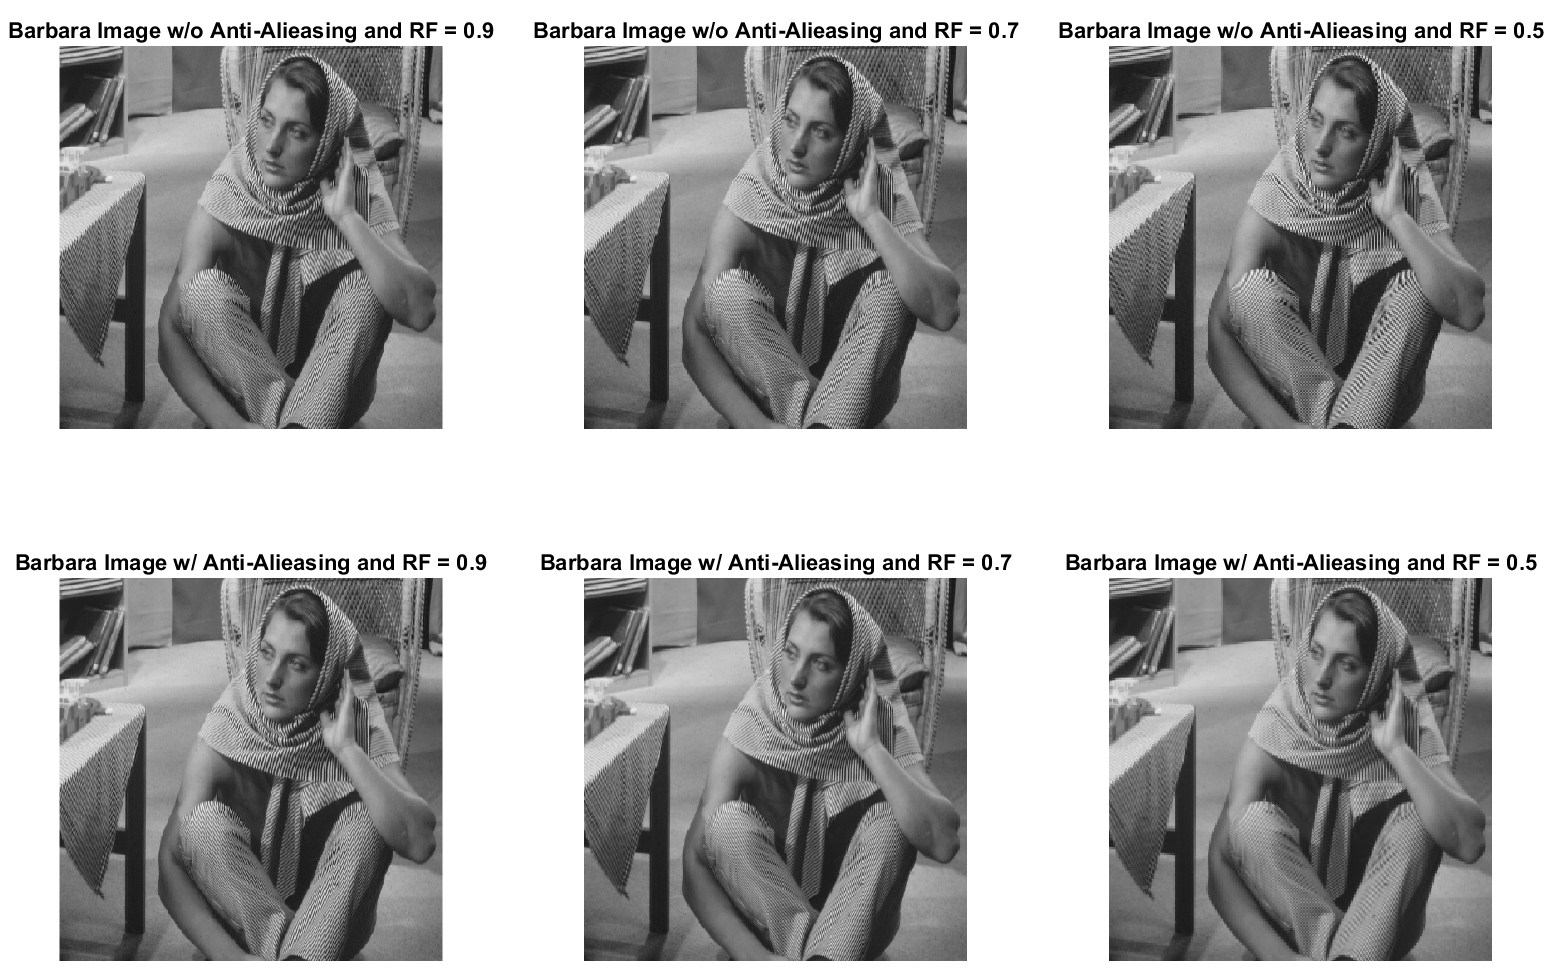
\includegraphics[width=13.5cm]{images/q4_c.png}
  \caption{\textit{barbaraLarge.jpg} displayed through the above script alongside its colorbar.}
\end{figure}
In the six images above, the effects of the resizing factor (\textit{rf}) and anti-aliasing were clearly visible. In 
the top row, without anti-aliasing, as the \textit{rf} gets further from 1 the clarity of the image decreases especially
in high-frequency areas, which are marked by dark or black pixels. For example, at \textit{rf} = 0.9, the image still 
maintains some of its original shape, but as the resize factor drops further to 0.7 or 0.5, the pixelation and jaggedness
become more pronounced. When antialiasing is applied, the high-contrast differences between neighboring pixels are 
smoothed out, reducing the appearance of jagged lines. However, in low-frequency areas, like the carpet behind Barbara,
there is almost no difference regardless of the resize factor or whether antialiasing is applied. The underlying cause
of these jagged lines and harsh contrasts is aliasing, which occurs when the sampling frequency is lower than the Nyquist
frequency, leading to high frequencies being misrepresented as lowerfrequencies. Antialiasing helps mitigate these
effects, producing smoother transitions, but reducing sharpness in high-contrast regions.

\hfill

\noindent In order to reduce the effects of aliasing, an image is often low-pass filtered before being resized or sampled.
The low pass filter removes high frequency components that are causing the aliasing, however this is at the cost of
details in the image. The script below was ran to show the effects of low-pass filtering on aliasing:
\begin{lstlisting}[style=Matlab-editor, basicstyle=\small\ttfamily]
  I=imread('barbaraLarge.jpg');
  % Low pass filtering before downsampling
  filt=fspecial('average',[3 3]);                 % creates a 3x3 low pass filter kernel
  filt_img=imfilter(I,filt,'conv');               % applies the lpf by convolving the image with the filter kernel
  
  B_LPF=imresize(filt_img, 0.7 , 'nearest');
  B=imresize(I, 0.7, 'nearest');
  
  figure,  imshow(I); title('Original Barbara Image');
  figure,  imshow(B); title('Barbara Image resized by 70% of original size');
  figure,  imshow(B_LPF); title('Low pass filter applied before Resizing to 70% of original size');
\end{lstlisting}
\begin{figure}[H]
  \centering
  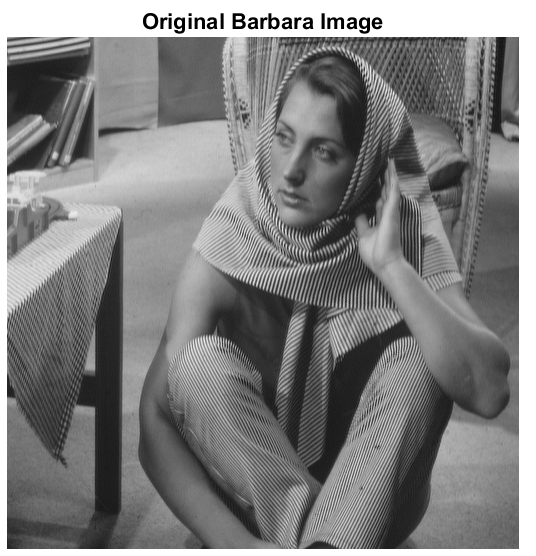
\includegraphics[width=5cm]{images/q4_e1.png} \\
  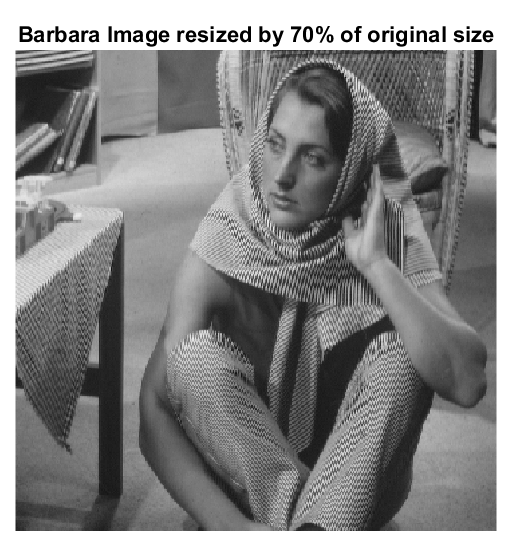
\includegraphics[width=5cm]{images/q4_e2.png}
  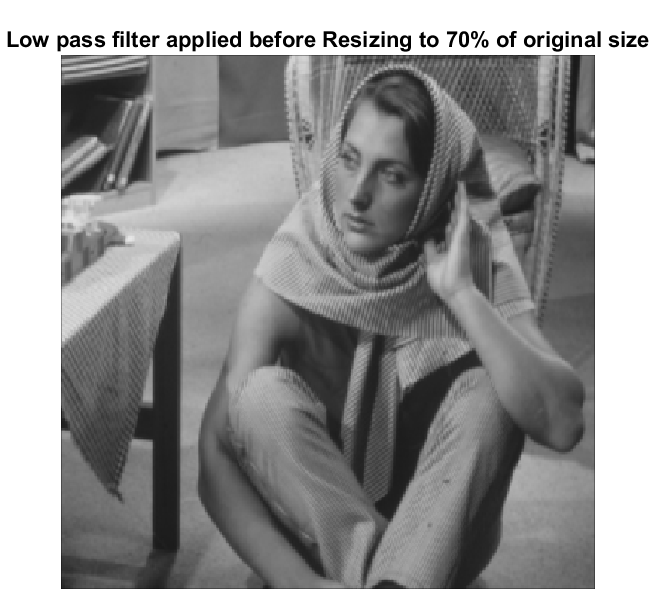
\includegraphics[width=6cm]{images/q4_e3.png}
  \caption{Results from the provided script above, displaying the effects of a low-pass filter on aliasing.}
\end{figure}
\end{document}